\chapter{Studi Pustaka}
\section{Twitter}
Twitter adalah sebuah jaringan informasi yang terdiri dari pesan-pesan sepanjang 140 karakter yang disebut \textit{tweet} \cite{TwitterDef:2015}. Pengguna Twitter di Indonesia terutama di kota Bandung ternyata cukup aktif dalam menggunakan Twitter. Dalam data yang dirilis lembaga pemantau media sosial Semiocast ditunjukan pada gambar \ref{fig:num_post_tweet} ``Top 20 Cities by Number of posted tweets'' pengguna Twitter di Kota Bandung berada di posisi 5 dengan perkiraan 1.2 persen dari 10 miliar \textit{tweets} selama Juni 2012.
\begin{figure}
\centering
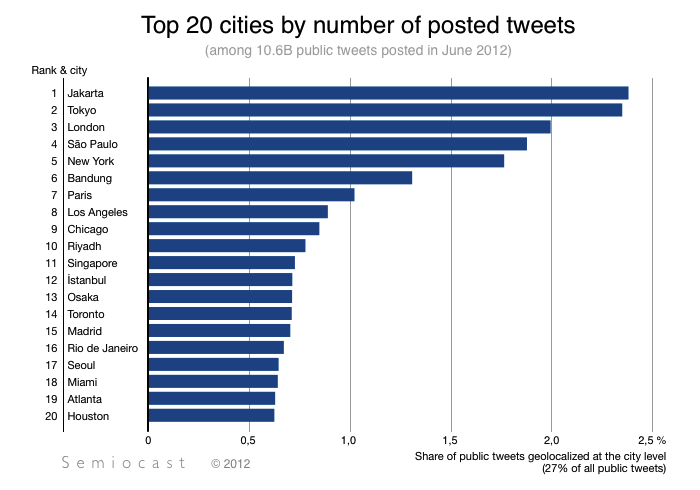
\includegraphics[width=\linewidth]{Gambar/mine/twittercity}
\caption[Top 20 cities by number of posted tweets, dari Semiocast]{Top 20 cities by number of posted tweets, dari Semiocast} 
\label{fig:num_post_tweet}
\end{figure}
Tingginya popularitas Twitter dapat dimanfaatkan untuk berbagai keperluan dalam berbagai aspek. Contohnya sebagai sarana komunikasi, memberikan opini, kampanye poilitik, bisnis, mendapatkan informasi, dan banyak lainya.
\section{Twitter API}
API (Application Programming \textit{interface}) merupakan sebuah cara yang didefinisikan sebuah program untuk menyelesaikan sebuah tugas, biasanya dengan menerima atau memodifikasi data \cite{TwitterApi:2015}. Twitter menyediakan sebuah API yang memberikan hak akses kepada pengembang perangkat lunak untuk membaca dan menulis data dari \textit{server}  Twitter. \textit{Programmer} menggunakan Twitter API untuk membuat aplikasi, \textit{website}, \textit{widgets}, dan proyek lainya yang berinteraksi dengan Twitter. Program akan berkomunikasi dengan Twitter API melalui HTTP. Twitter menyediakan beberapa jenis dan fungsi API yang berbeda, diantaranya REST API, Streaming API, dan ads API.
\subsection{REST API}
REST API menyediakan akses secara program untuk membaca dan menulis data Twitter. Beberapa akses yang disediakan oleh Twitter seperti membuat \textit{tweet} baru, membaca profil \textit{author}, data \textit{follower} dan lain-lain \cite{RESTAPI:2015}. REST API mengidentifikasi aplikasi dan pengguna Twitter menggunakan OAuth. Twitter menyarankan jika pengembang berniat untuk memonitor atau memproses \textit{tweets} secara \textit{real-time} lebih baik menggunakan Streaming API daripada REST API, dikarenakan REST API memiliki \textit{rate limits}.\\\\
\textit{Rate limiting} pada API versi 1.1 ditujukan per-\textit{user} basis atau per \textit{access token}. \textit{Rate limits} pada API versi 1.1 dibagi kedalam selang 15 menit. Ada 2 buah kelompok GET \textit{request} : 15 panggilan setiap 15 menit, dan 180 panggilan setiap 15 menit. Setiap \textit{endpoints} membutuhkan autentikasi. Ini bertujuan agar mencegah kebiasaan yang buruk, dan juga dapat membantu Twitter mengerti lebih jauh bagaimana mengkategorikan aplikasi yang menggunakan API.
\subsection{Streaming API}
Streaming API memberikan latensi yang rendah kepada pengembang untuk mengakses Twitter \textit{global stream} dari data \textit{tweets}. Pengimplementasian secara tepat dan benar dapat menghindari \textit{overhead}. Twitter menawarkan beberapa \textit{streaming endpoints}, setiap \textit{endpoints} telah disesuaikan untuk kasus tertentu \cite{StreamingAPI:2015}.
\begin{enumerate}
	\item \textit{Public Streams}\\
	\textit{Public Stream} menyediakan data publik yang mengalir melewati Twitter. Jenis ini cocok untuk memantau spesifik \textit{user} atau topik, dan penambangan data.
	\item \textit{User Streams}\\
	\textit{User Streams} menyediakan aliran data dan spesifik kejadian untuk \textit{user} yang terautentikasi. \textit{User Streams} tunggal, mengandung semua data yang sesuai dengan \textit{view} yang dimiliki \textit{user} tunggal dari Twitter. 
	\item \textit{Site Streams}\\
	\textit{Site Streams} adalah versi beberapa \textit{user} dari \textit{User Streams}. \textit{Site stream} ditujukan untuk \textit{server}  yang terhubung ke Twitter atas nama banyak \textit{user}. \textit{Site streams} berguna untuk menerima \textit{udates} secara \textit{real-times} dari jumlah \textit{user} yang banyak. 
\end{enumerate}
\subsection{Perbedaaan antara Streaming dan REST}
Streaming API dan REST API memiliki beberapa perbedaan. Karena adanya perbedaan ini, pengembang harus memikirkan jenis API mana yang cocok digunakan dalam aplikasinya. Setiap API memiliki karakteristik dan kelebihan yang berbeda-beda \cite{StreamingAPI:2015}.\\\\
Pada Streaming API, aplikasi memerlukan koneksi HTTP yang tetap terbuka antara \textit{streaming process} dengan \textit{server}  Twitter. Streaming API tidak dapat merespon permintaan \textit{user} secara langsung, namun \textit{user} \textit{request} harus ditangani oleh HTTP \textit{server}  yang dimiliki oleh aplikasi. Pada gambar \ref{fig:stream_api}, aplikasi memiliki 2 buah penanganan yang terdiri dari \textit{server}  yang menangani \textit{user} \textit{request}, dan \textit{server}  yang menangani \textit{streaming process}.\\\\
\begin{figure}
\centering
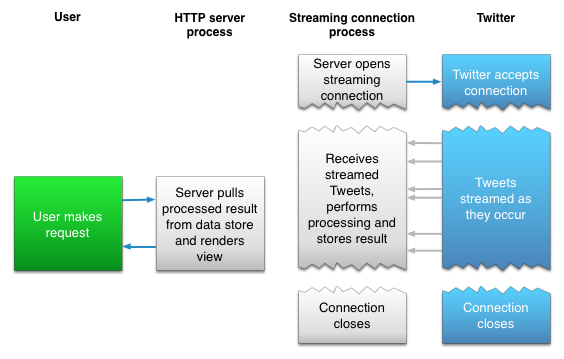
\includegraphics[width=\linewidth]{Gambar/mine/streamingapi}
\caption[Streaming API \textit{Architecture}, dari \cite{StreamingAPI:2015}]{Streaming API \textit{Architecture}, dari \cite{StreamingAPI:2015}} 
\label{fig:stream_api}
\end{figure}
Dalam menggunakan REST API aplikasi idealnya memiliki 2 buah koneksi HTTP. Koneksi \textit{user} dengan HTTP \textit{server}  dan Twitter \textit{server}  dengan HTTP \textit{server}. Permintaan \textit{user} akan diteruskan oleh HTTP \textit{server}  melalui REST API ke \textit{server}  Twitter. Respon dari \textit{server}  Twitter akan diproses oleh HTTP \textit{server}  dan diteruskan kepada \textit{user}. Gambar \ref{fig:rest_api} menggambarkan cara kerja dari REST API.\\
\begin{figure}
\centering
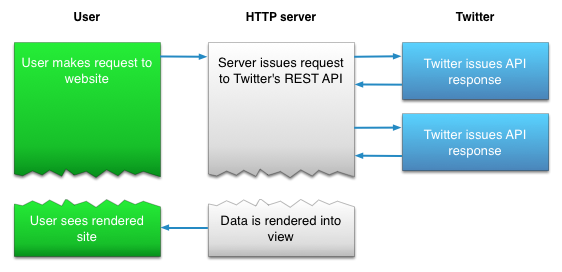
\includegraphics[width=0.8\linewidth]{Gambar/mine/restapi}
\caption[REST API \textit{Architecture}, dari \cite{RESTAPI:2015}]{REST API \textit{Architecture}, dari \cite{RESTAPI:2015}} 
\label{fig:rest_api}
\end{figure}
\section{OAuth}
OAuth 2.0 \textit{authorization} adalah sebuah \textit{framework} yang memungkinkan sebuah aplikasi pihak ke-tiga untuk mendapatkan akses terbatas pada layanan HTTP, tanpa memberikan data autentikasi \cite{RFCOAuth:2012}. Dalam model tradisional autentikasi \textit{client}-server, ketika \textit{client} meminta \textit{requests} sebuah akses terhadap sumber daya yang dilindungi, pemilik dari sumber daya harus memberikan surat kepercayaan kepada \textit{client}. Dalam hal mendukung aplikasi pihak ke-3, pemilik sumber daya harus membagi surat kepercayaanya kepada pihak ke-3. Hal ini menyebabkan beberapa masalah dan batasan : 
\begin{enumerate}
	\item Aplikasi pihak ke-3 perlu menyimpan surat kepercayaan pemilik sumber daya untuk penggunaan dimasa depan, biasanya adalah sebuah textit{password} dalam teks.
	\item \textit{Server}  perlu mendukung autentikasi \textit{password}, walaupun kelemahan keamanan melekat pada \textit{passwords}.
	\item Aplikasi pihak ke-3 mendapatkan seluruh akses pada sumber daya yang dilindungi. Pemilik sumber daya tidak bisa memberikan batasan akses kepada pihak ke-3.
	\item Pemilik sumber daya tidak bisa mencabut akses aplikasi pihak ke-3 tanpa mencabut seluruh akses pihak ke-3, dan harus mengganti password.
\end{enumerate}
OAuth mengatasi masalah ini dengan memperkenalkan sebuah \textit{author}ization \textit{layer} dan membagi peran \textit{client} untuk mengakses sumber daya. Sebagai ganti menggunakan surat kepercayaan pemilik untuk mengakses sumber daya yang dilindungi. \textit{Client} mendapatkan \textit{access token} (sebuah string yang berisi cakupan yang spesifik, waktu akses, dan attribut akses lainya.) \textit{access token} diberikan kepada \textit{client} atau pihak ketiga oleh \textit{author}ization \textit{server}  dengan persetujuan pemiliki sumber daya. \textit{Client} menggunakan \textit{access token} untuk mengakses sumber daya yang dilindungi oleh \textit{resource server}.\\\\
Dalam OAuth didefinisikan ada 4 peran:
\begin{enumerate}
	\item Resource Owner\\
	Sebuah entitas yang dapat memberika akses kepada sumber daya yang dilindungi. Ketika resource owner seorang manusia, ini merujuk pada end-\textit{user}.
	\item Resource Server\\
	\textit{server}  yang menyediakan sumber daya yang dilindungi, dapat menerima dan merespon permintaan sumber daya yang dilindungi menggunakan \textit{access token}s.
	\item \textit{client}\\
	Sebuah aplikasi yang meminta hak akses kepada sumber daya yang dilindungi.
	\item \textit{authorization server}\\
	\textit{server}  yang memberikan \textit{access token}s kepada \textit{client} ketika proses autentikasi berhasil.
\end{enumerate}
\textit{Protocol Flow} dari Oauth akan dijelaskan pada gambar 2.4\\
\begin{figure}
\centering
\includegraphics[width=0.8\linewidth]{Gambar/mine/OAuth}
\caption[\textit{Protocol Flow} Oauth, dari \cite{RFCOAuth:2012}]{\textit{Protocol Flow} Oauth, dari \cite{RFCOAuth:2012}} 
\label{fig:oauth_flow_protocol}
\end{figure}
\begin{enumerate}
	\item \textit{client} melakukan meminta \textit{authorization grant} kepada pemiliki sumber daya. Permintaan bisa dilakukan secara langsung kepada pemilik sumber daya, atau secara tidak langsung melewati \textit{authorization server}  sebagai penengah.
	\item \textit{client} mendapatkan \textit{author}ization grant.
	\item \textit{authorization grant} digunakan untuk meminta \textit{access token} kepada \textit{author}ization Server.
	\item \textit{authorization server}  mengautentikasi apakah \textit{authorization grant} yang dimiliki \textit{client} valid, dan jika valid, \textit{client} diberikan sebuah \textit{access token}.
	\item \textit{client} meminta sumber daya yang dilindungi dari sumber daya \textit{server}  dan melakukan autentikasi dengan memperlihatkan \textit{acces token}.
	\item \textit{resource server}  memvalidasi \textit{access token}, dan jika valid, \textit{server}  akan melayani permintaan.
\end{enumerate}
\section{Twitter4J}
Twitter4j adalah sebuah Java library untuk Twitter API bersifat \textit{open source} dan gratis. Dengan Twitter4j, \textit{user} dapat dengan mudah mengintegrasikan aplikasi Java dengan Twitter service. Twitter4j dapat di unduh pada situs \url{http://twitter4j.org} \cite{Twitter4j:2015}. Berikut beberapa kelas yang dimiliki oleh Twitter4j:\\\\
\textbf{Twitter} adalah sebuah \textit{interface} yang digunakan untuk membungkus Twitter REST API. Method yang dimiliki kelas ini sebagai berikut:
\begin{enumerate}
	\item \textbf{TimelinesResources timelines()}\\
	Berfungsi mendapatkan objek TimelinesResources\\
	\textbf{Kembalian} Mengembalikan sumber daya berupa \textit{timelines} yang dimiliki oleh pemilik sumber daya berdasarkan \textit{access token} Oauth.
	\item \textbf{TweetsResources tweets()}\\
	Berfungsi mendapatkan objek TweetResources\\
	\textbf{Kembalian} Mengembalikan sumber daya berupa \textit{tweets} yang dimiliki oleh pemilik sumber daya berdasarkan \textit{access token} Oauth.
	\item \textbf{SearchResource search()}\\
	Berfungsi mendapatkan objek SearchResource\\
	\textbf{Kembalian} Mengembalikan kelas SearchResource yang dimiliki oleh pemilik sumber daya berdasarkan \textit{access token} Oauth.
\end{enumerate}
\textbf{TwitterFactory} adalah sebuah kelas denggan pattern singleton yang digunakan untuk menginstansiasi kelas Twitter berdasarkan \textit{config tree}. Method yang dimiliki kelas ini sebagai berikut:
\begin{enumerate} 
	\item \textbf{static Twitter getSingleton()}\\
	Berfungsi menginstansiasi kelas Twitter hanya satu kali.\\
	\textbf{Kembalian} instansiasi default singleton Twitter 
\end{enumerate}
\textbf{TwitterStream} adalah sebuah \textit{interface} yang digunakan untuk membungkus Twitter Streaming API. Method yang dimiliki kelas ini sebagai berikut:
\begin{enumerate}
	\item \textbf{void addListener(StreamListener listener)}\\
	Berfungsi menambahkan \textit{listener}.\\
	\textbf{Kembalian} void
	\item \textbf{void removeListener(StreamListener listener)}\\
	Berfungsi menghapus \textit{listener}.\\
	\textbf{Kembalian} void
	\item \textbf{void filter(String query)}\\	
	Berfungsi mengkonsumsi status publik yang sesuai dengan satu atau lebih predikat \textit{filter}.\\
	\textbf{parameter} query - String\\
	\textbf{Kembalian} void
	\item \textbf{void shutdown()}\\
	Berfungsi mematikan thread yang dibagikan oleh instansiasi TwitterStream\\
	\textbf{Kembalian} void
\end{enumerate}
\textbf{TwitterStreamFactory} adalah sebuah kelas yang digunakan untuk menginstansiasi kelas TwitterStream. Method yang dimiliki kelas ini sebagai berikut:
\begin{enumerate}
	\item \textbf{static TwitterStream getSingleton()}\\
	Berfungsi mendapatkan instansiasi dari kelas TwitterStream\\
	\textbf{Kembalian} instansiasi default singleton TwitterStream
\end{enumerate}
\textbf{Paging} adalah sebuah kelas yang digunakan untuk mengontrol \textit{pagination}. Method yang dimiliki kelas ini sebagai berikut:
\begin{enumerate}
	\item \textbf{void setCount(int count)}\\
	Berfungsi untuk mengubah banyaknya status dalam 1 page\\
	\textbf{Parameter} count - int\\
	\textbf{Kembalian} void
	\item \textbf{void setPage(int page)}\\
	Berfungsi untuk mengubah nomor page yang dipilih\\
	\textbf{Parameter} page - int\\
	\textbf{Kembalian} void
\end{enumerate}
\textbf{TimelinesResources} adalah sebuah kelas yang digunakan untuk mengolah timelines berdasarkan hak akses dari \textit{access token}. Method yang dimiliki kelas ini sebagai berikut:
\begin{enumerate}
	\item \textbf{ResponseList<Status> getUserTimeline(String screenName,Paging paging)}\\
	Berfungsi untuk mendapatkan status dari timeline seseorang sejumlah paging yang diinginkan.\\
	\textbf{Parameter} screenName - String, paging - Paging\\
	\textbf{Kembalian} status dari timeline spesifik \textit{user}.
\end{enumerate}
\textbf{SearchResources} adalah sebuah kelas yang digunakan untuk mengolah pencarian berdasarkan hak akses dari \textit{access token}. Method yang dimiliki kelas ini sebagai berikut:
\begin{enumerate}
	\item \textbf{QueryResult search(Query query)}\\
	Berfungsi untuk mendapatkan tweets yang sesuai dengan spesifik query.\\
	\textbf{Parameter} query - Query\\
	\textbf{Kembalian} result dari query diminta
\end{enumerate}
\textbf{Query} adalah sebuah kelas yang digunakan untuk mengolah query untuk menentukan pencarian. Method yang dimiliki kelas ini sebagai berikut:
\begin{enumerate}
	\item \textbf{void setGeoCode(GeoLocation location, double radius, Unit unit}\\
	Berfungsi untuk mencari \textit{tweets} berdasarkan radius tertentu.\\
	\textbf{Parameter} location - GeoLocation, radius - doouble, unit - Query.Unit)\\
	\textbf{Kembalian} void
	\item \textbf{void setLocale(String locale)}\\
	Berfungsi untuk mencari \textit{tweets} hanya pada bahasa tertentu.\\
	\textbf{Parameter} locale - String\\
	\textbf{Kembalian} void
	\item \textbf{void setSince(String since)}\\
	Berfungsi untuk mencari \textit{tweets} sejak tanggal tertentu.\\
	\textbf{Parameter} since - String\\
	\textbf{Kembalian} void
\end{enumerate}
\textbf{Status} adalah sebuah \textit{interface} yang merepresentasikan sebuah status dari seorang \textit{user}. Method yang dimiliki kelas ini sebagai berikut:
\begin{enumerate}
	\item \textbf{java.util.Date getCreatedAt()}\\
	Berfungsi untuk mengetahui tanggal status tersebut dibuat.\\
	\textbf{Kembalian} tanggal status dibuat.
	\item \textbf{long getId()}\\
	Berfungsi untuk mengetahui id status tersebut.\\
	\textbf{Kembalian} id status.
	\item \textbf{java.lang.String getText()}\\
	Berfungsi untuk mengambil isi dari status.\\
	\textbf{Kembalian} isi dari status
	\item \textbf{GeoLocation getGeoLocation()}\\
	Berfungsi untuk mengetahui lokasi tweet bila diketahui.\\
	\textbf{Kembalian} lokasi tweets berasa jika lokasi diketahui.
	\item \textbf{User getUser()}\\
	Berfungsi untuk mengetahui user yang terasosiasi dengan status.\\
	\textbf{Kembalian}user yang terasosiasi dengan status.
\end{enumerate}
\textbf{StatusListener} adalah sebuah \textit{interface} yang merepresentasikan bagaimana status yang dilisten akan ditangani. Method yang dimiliki kelas ini sebagai berikut:
\begin{enumerate}
	\item \textbf{void onDeletion}\\
	Berfungsi menangani ketika \textit{deletionNotices} disampaikan.\\
	\textbf{Kembalian} void.
	\item \textbf{void onStatus}\\
	Berfungsi menangani ketika mendapatkan status ketika melakukan proses \textit{listen}.\\
	\textbf{Kembalian} void.
\end{enumerate}
\section{Jaringan Saraf Tiruan}
Jaringan Saraf Tiruan (JST) adalah paradigma memproses sebuah informasi yang terinspirasi dari cara kerja sistem saraf biologi, seperti otak, memproses informasi \cite{WhatisNN:2015}. Kunci utama dari paradigma ini adalah struktur dari sistem proses informasi. Sistem ini terdiri dari dari banyak unsur proses yang saling terhubung (neuron) bekerja secara serempak untuk menyelesaikan suatu masalah.  JST dikonfigurasi untuk sebuah penerapan yang spesifik, seperti  pengenalan pola atau pengklasifikasian data, melalui proses belajar. Di dalam sistem biologi, belajar melibatkan penyesuaian hubungan sinaptik yang berada diantara neuron.\\\\
Dalam sub bab dibawah peneliti akan membahas beberapa hal mengenai Jaringan Saraf Tiruan meliputi :
\begin{enumerate}
	\item \textbf{Cara Kerja Jaringan Saraf Biologi}, untuk mengerti JST bekerja kita harus mengetahui cara kerja dari jaringan saraf biologi itu sendiri, dalam sub bab ini akan dibahas mengenai jaringan saraf biologi.
	\item \textbf{Masalah yang tidak cocok diselesaikan dengan JST}, dalam sub bab ini akan dibahas bagaimana JST bisa menyelesaikan masalah
	\item \textbf{Masalah yang dapat diselesaikan dengan JST}, dalam sub bab ini akan dibahas jenis permasalahan yang efektif dikerjakan oleh JST
	\item \textbf{Metode Pembelajaran}, agar JST dapat menyelesaikan suatu masalah diperlukan proses belajar seperti halnya jaringan saraf biologi. Bab ini akan membahas metode pembelajaran.
	\item \textbf{Perhitungan Galat}, dalam bab ini akan dibahas cara menghitung galat dari masukan dan keluaran JST.
	\item \textbf{Feedforward Neural Network}, pada bab ini akan dibahas jenis JST yang bernama Feedforward Neural Network.
\end{enumerate}
\subsection{Cara Kerja Jaringan Saraf Biologi}
Untuk membangun sebuah komputer yang dapat berfikir seperti manusia, para
peneiliti harus memodelkanya seperti otak manusia. Komposisi utama otak
manusia adalah sel neuron. JST harus mencoba mensimulasikan sifat-sifat dari
sel neuron itu sendiri.\\\\
Sebuah sel neuron, seperti pada gambar \ref{fig:neuron_biologi}, menerima sinyal dari dendrit. Ketika neuron menerima sebuah sinyal, ada kemungkinan neuron tersebut meneruskan sinyal tersebut. Ketika neuron meneruskanya, sinyal tersebut ditransimisikan melewati axon neuron. Sinyal tersebut akan melewati terminal axon, dan ditransmisikan ke neuron lain.
\begin{figure}
\centering
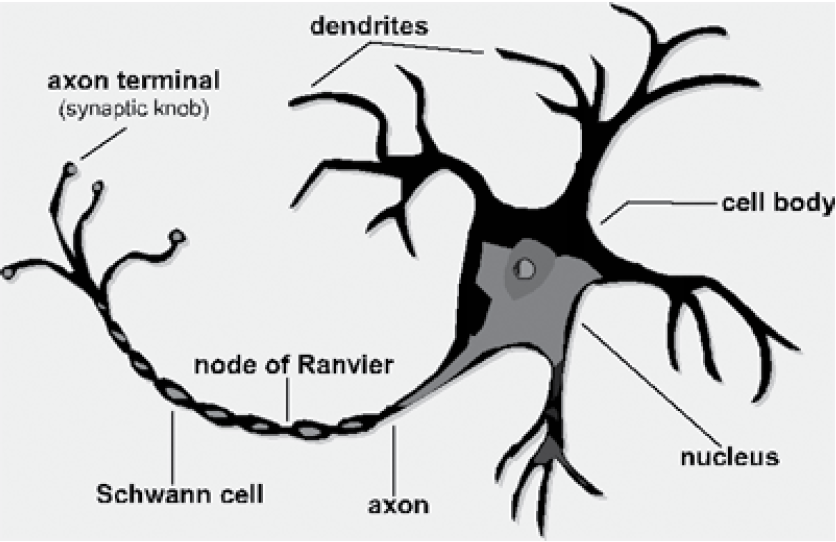
\includegraphics[width=0.7\linewidth]{Gambar/mine/neuron}
\caption[Neuron Biologi, dari \cite{IntroNNforJava:2015}]{Neuron Biologi, dari \cite{IntroNNforJava:2015}} 
\label{fig:neuron_biologi}
\end{figure}
\subsection{Masalah yang tidak cocok diselesaikan dengan JST}
JST dapat memproses kumpulan informasi yang akan menghasilkan keluaran. Keluaran JST nantinya akan digunakan untuk membantu pengambilan sebuah keputusan. Faktanya tidak semua masalah cocok diselesaikan dengan JST. Ada beberapa jenis masalah yang kurang cocok diselesaikan oleh JST :
\begin{enumerate}
	\item Masalah yang dapat diselesaikan dengan program yang mudah untuk di tuliskan kedalam \textit{flowcharts}.
	\item Masalah yang dapat diselesaikan dengan program yang langkahnya dapat didefnisikan dengan terperinci.
	\item Masalah yang harus diketahui cara solusinya diturunkan.
	\item Algoritma yang digunakan untuk menyelesaikan sebuah masalah tidak berubah-rubah (Statik).
\end{enumerate}
\subsection{Masalah yang dapat diselesaikan dengan JST}
Walau tidak semua masalah dapat diselesaikan oleh JST, namun ada banyak hal yang dapat diselesaikan oleh JST. Jenis masalah yang sering diselesaikan oleh JST sebagai berikut :
\begin{enumerate}
	\item \textbf{Classification} adalah proses mengklasifikasian informasi menjadi beberapa
jenis kelompok. Contohnya, perusahaan asuransi ingin mengklasifikasikan permohononan asuransi menjadi beberapa kategori risiko yang berbeda, atau sebuah organisasi online ingin membuat sistem email mereka dapat mengklasifikasikan pesan masuk menjadi kelompok \textit{spam} dan bukan \textit{spam}. Untuk mencapai hal tersebut JST harus dilatih menggunakan beberapa contoh kelompok data dan instruksi. Setiap kelompok data diklasifikasikan menjadi anggota himpunan tertentu. JST dapat belajar dari contoh kelompok data tersebut. Setelah proses pembelajaran diharapkan JST dapat mengindikasi anggota kelompok data yang baru.
	\item \textbf{Prediction} adalah penerapan lain yang sering digunakan untuk JST. Dengan memberikan serangkaian masukan-keluaran data berdasarkan basis waktu, sebuah JST
digunakan untuk memprediksi masa depan. Akurasi prediksi akan bergantung pada banyak faktor, seperti quantiti dan relevansi dari masukan data. JST biasanya diterapkan pada masalah yang melibatkan prediksi pergerakan dalam pasar finansial.
	\item \textbf{Pattern Recognition} adalah sebuah bentuk pengklasifikasian. Pattern recognition adalah kemampuan untuk mengenali pola. Pola harus bisa dikenali bahkan ketika datanya berubah. Sebagai contoh dalam kehidupan kita pengemudi harus dapat dengan tepat mengidentifikasi lampu lalu lintas. Walaupun tidak semua lampu stopan bentuknya sama, pengemudi tetap dapat mengenalinya. Hal ini juga harus dicapai oleh JST agar komputer dapat melakukan pengenalan pola.
	\item \textbf{Pattern Recognition} adalah sebuah bentuk pengklasifikasian. Pattern recognition adalah kemampuan untuk mengenali pola. Pola harus bisa dikenali bahkan ketika datanya berubah. Sebagai contoh dalam kehidupan nyata, pengemudi harus dapat dengan tepat mengidentifikasi lampu lalu lintas. Walaupun tidak semua lampu stopan bentuknya sama, pengemudi tetap dapat mengenalinya. Hal ini juga harus dicapai oleh JST agar komputer dapat melakukan pengenalan pola.
	\item \textbf{Optimization} suatu kemampuan JST untuk mencari solusi yang optimal. Biasanya digunakan ketika suatu masalah memiliki \textit{state space} yang sangat besar. JST mungkin tidak selalu menemukan solusi optimal, namun JST dapat mencari solusi yang dapat diterima. Salah satu masalah optimasi yang paling terkenal ialah Traveling Sales Problem.
\end{enumerate}
\subsection{Metode Pembelajaran}
Ada banyak cara untuk membuat JST dapat belajar. Setiap algoritma pembelajaran nantinya akan melibatkan perubahan bobot setiap penghubung neuron. Proses pelatihan sangatlah penting bagi JST. Ada dua bentuk dari pelatihan yang dapat digunakan,\textit{ supervised }dan \textit{unsupervised}.\textit{ supervised training}melibatkan JST dengan serangkaian masukan-keluaran yang diinginkan. Pada \textit{unsupervised training} dibutuhkan juga kumpulan pelatihan, namun pelatihan tersebut tidak perlu disertai keluaran.
\begin{enumerate}
	\item \textit{Unsupervised training} adalah salah satu metode pembelajaran yang disediakan data masukan namun tidak perlu disediakan antisipasi keluaran. \textit{Unsupervised training} biasanya digunakan untuk melatih JST klasifikasi. Penerapan lainya digunakan untuk data mining. \textit{Unsupervised training} juga biasa digunakan untuk \textit{self-organizing maps} (SOM). \textit{Unsupervised training} dapat diterapkan kedalam banyak situasi. Pada gambar \ref{fig:uns_learning} dijelaskan \textit{flowcharts} proses \textit{unsupervised training}.\\
	
	\begin{figure}
\centering
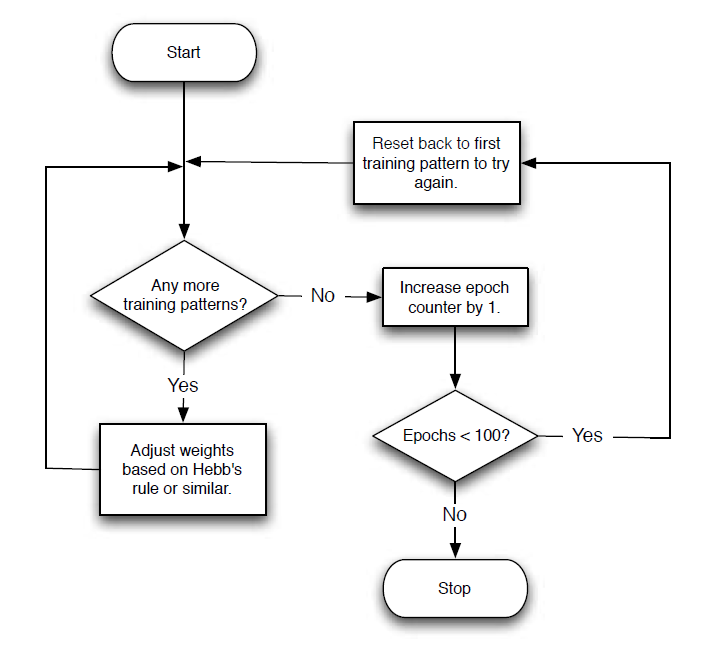
\includegraphics[width=0.8\textwidth]{Gambar/mine/unsupervised}
\caption[\textit{Unsupervised training}, dari \cite{IntroNNforJava:2015}]{\textit{Unsupervised training}, dari \cite{IntroNNforJava:2015}} 
\label{fig:uns_learning}
\end{figure}
	\item \textit{Supervised Training} adalah metode pembelajaran, yang memiliki sekumpulan pelatihan. Perbedaan utama antara\textit{ supervised training} dan \textit{unsupervised training} adalah pada\textit{ supervised training} disediakan harapan keluaran. Hal ini memungkinkan JST untuk menyesuaikan nilai dari bobot matriks  berdasarkan perbedaan antara keluaran yang diharapkan dengan keluaran yang sesunguhnya. Pada gambar \ref{fig:s_learning} dijelaskan \textit{flowcharts} proses \textit{supervised training}.\\\\
	\begin{figure}
	\centering
	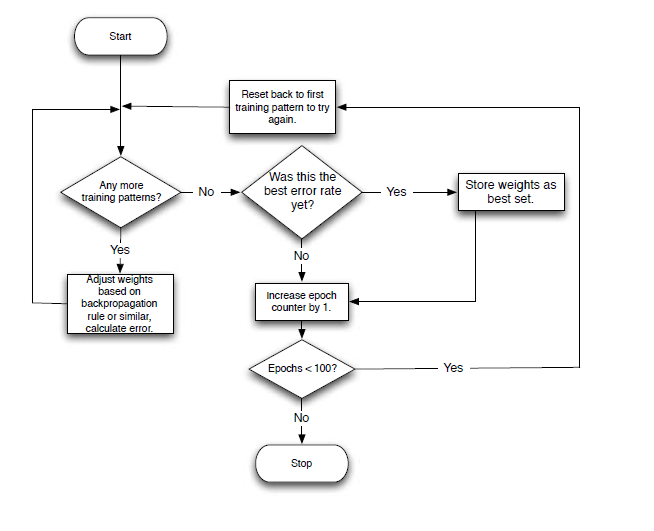
\includegraphics[width=0.8\textwidth]{Gambar/mine/supervised}
	\caption[\textit{Supervised training}, dari \cite{IntroNNforJava:2015}]{\textit{Supervised training}, dari \cite{IntroNNforJava:2015}} 
	\label{fig:s_learning}
	\end{figure}
\end{enumerate}
\subsection{Perhitungan Galat}
Perhitungan galat adalah salah satu aspek penting dari setiap pelatihan JST. Apakah pelatihan itu adalah\textit{ supervised }atau \textit{unsupervised}, sebuah rata-rata galat harus dihitung. Tujuan dari setiap algoritma pelatihan ialah untuk meminimalisasi rata-rata galat.
\subsubsection{Perhitungan Galat dan\textit{ supervised }Training}
Ada dua nilai yang harus dipertimbangkan dalam menentukan rata-rata galat untuk\textit{ supervised training}. Pertama kita harus menghitung galat untuk setiap element pelatihan. Kedua, kita harus menghitung rata-rata galat untuk semua element pelatihan untuk setiap sampel. (Root Mean Square) RMS adalah salah satu metode untuk menghitung rata-rata galat untuk sebuah pelatihan. Metode RMS efektif dalam perhitungan rata-rata galat, tanpa memperhatikan apakah hasil yang sebenarnya lebih tinggi atau lebih kecil daripada hasil yang diharapkan. Untuk menghitung RMS digunakan formula. 
\begin{displaymath}
	x_{rms}= \sqrt{\frac{1}{n}\sum_{i=1}^{n}(aktual_{i}-ideal_{i})^2}	
\end{displaymath}
Dimana n adalah jumlah pasangan masukan dan keluaran, aktual adalah keluaran yang dihasilkan oleh JST, dan ideal adalah keluaran yang diinginkan. Dengan mengetahui rata-rata galat dari keluaran yang diharapkan dan yang sebenarnya, kita dapat menentukan apakah JST tersebut sudah cukup baik atau belum.
\subsection{Feedforward Neural Network}
Feedforward adalah sebuah arsitektur JST yang populer dan banyak digunakan sebagai model dalam banyak penerapan. Feedforward dikenal juga sebagai ``multi-layer perceptron''. Dalam JST feedforward, setiap layer dari JST mengandung hubungan ke layer berikutnya (contohnya dari layer masukan dihubungkan ke layer tersembunyi) ilustrasi feedforward pada gambar \ref{fig:ffnn}. Hubungan antar neuron pada feedforward hanya satu arah. Feedfoward selalu dimulai dari layer masukan. Jika masukan terhubung dengan sebuah layer tersembunyi, layer tersembunyi dapat terhubung dengan layer tersembunyi lainya atau dapat langsung terhubung dengan layer keluaran. Jumlah layer tersembunyi bisa banyak. Kebanyakan JST biasanya akan memiliki satu buah layer tersembunyi, dan akan sangat jarang JST memiliki lebih dari dua buah layer tersembunyi.\\
\begin{figure}
	\centering
	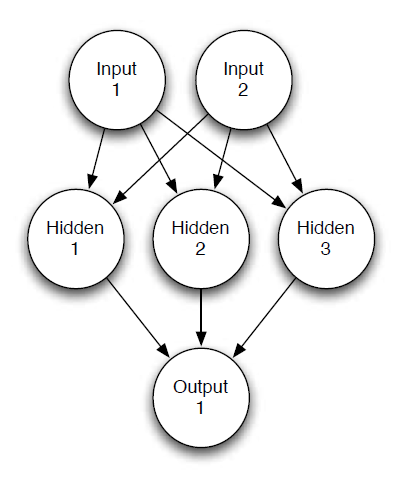
\includegraphics[width=0.6\linewidth]{Gambar/mine/ffnn}
	\caption[Contoh Feed Forward Neural Network, dari \cite{IntroNNforJava:2015}]{Contoh Feed Forward Neural Network, dari \cite{IntroNNforJava:2015}} 
	\label{fig:ffnn}
	\end{figure}
\textbf{Memilih Struktur Jaringan}\\
Ada banyak cara untuk membangun JST feedforward. Kita harus menentukan berapa jumlah neuron pada layer masukan dan layer keluaran. Selain itu layer tersembunyi harus ditentukan. Ada banyak teknik untuk memilih parameter tersebut. Untuk menentukan struktur yang optimal pada feedforward dibutuhkan pengalaman dan percobaan.
\begin{enumerate}
\item\textbf{Layer masukan}\\Jumlah neuron pada layer masukan dapat ditentukan bergantung pada data yang kita miliki. Parameter ini biasanya ditentukan secara unik ketika kita mengetahui data pelatihan kita. Secara spesifik, jumlah dari neuron setara dengan banyaknya kolum pada data kita. Biasanya kita dapat menambahkan satu buah titik bias.
\item\textbf{Layer Keluaran}\\Seperti layer masukan, setiap JST memiliki satu buah layer keluaran. Untuk jumlah neuron di dalamanya ditentukan pada model apa yang kita gunakan. Apakah JST kita \textit{Machine Mode} atau \textit{Regression Mode}. Jika pada \textit{Machine Mode} JST akan mengembalikan kelas, sedangkan pada \textit{Regression Mode} mengembalikan sebuah nilai. bila JST menggunakan sebuah regressor, maka keluarannya akan memiliki 1 neuron. Bila keluarannya sebuah pengklasifikasian, maka akan memiliki satu neuron atau lebih.
\item\textbf{Layer Tersembunyi}\\Dalam menentukan layer tersembunyi ada dua buah keputusan yang harus diperhatikan. Pertama menentukan berapa jumlah layer tersembunyi yang dibutuhkan. Kedua menentukan berapa jumlah neuron pada setiap layer.\\\\ 
Secara teori tidak ada alasan untuk menggunakan layer tersembunyi lebih dari dua. Faktanya pada masalah yang ada pada kehidupan sehari-hari, dengan 1 buah layer tersembunyi banyak masalah dapat diselesaikan. Tabel \ref{table:jmlhHiddenLayer} merupakan kegunaan JST berdasarkan banyaknya layer tersembunyi\\\\
\begin{table}
\centering
\caption{Menentukan jumlah hidden layer}
\label{table:jmlhHiddenLayer}
\begin{tabular}{|l|p{12cm}|}
\hline
Jumlah Hidden Layer & Kegunaan \\\hline
tidak ada & Hanya dapat merepresentasikan fungsi linear atau pemilihan linear.\\\hline
1 & Dapat memeperikaran semua fungsi yang mengandung pemetaan kontinu dari satu \textit{space} terbatas ke yang lainya.\\\hline
2 & Dapat merepresentasikan sebuah keputusan yang  batasanya dan akurasi yang berubah-ubah dengan fungsi aktivasi rasional dan dapat memperkirakan setiap pemetaan halus untuk akurasi apapun.\\\hline
\end{tabular}
\end{table}
Untuk menentukan jumlah neuron dalam layer tersembunyi adalah bagian yang sangat penting dalam menentukan keseluruhan arsitektur JST. Walaupun layer ini tidak secara langsung berinteraksi dengan lingkungan luar, layer ini memiliki pengaruh yang sangat besar pada akhir keluaran. Jumlah layer tersembunyi dan jumlah neuronya sangat penting diperhatikan. Jika kita terlalu sedikit menggunakan neuron dalam layer tersembunyi ini akan mengakibatkan sesuatu yang disebut \textit{underfitting}. Namun bila terlalu banyak menggunakan neuron pada layer tersembunyi ini akan mengakibatkan \textit{overfitting}. \textit{Overfitting} terjadi ketika JST terlalu banyak memiliki informasi yang diproses daripada jumlah batas dari informasi yang terkandung dalam sejumlah pelatihan. Ada beberapa tips untuk menentukan jumlah neuron: Pertama jumlah neuron harus berada diantara jumlah masukan dan keluaran. Kedua jumlah neuron seharusnya 2/3 ukuran dari layer masukan, ditambah dengan layer keluaran. Ketiga jumlah neuron seharusnya kurang dari dua kali dari layer masukan.
\item\textbf{Fungsi Aktivasi}\\
Kebanyakakn JST mengeluarkan keluaran dari layernya menggunakan fungsi aktivasi. Fungsi aktivasi ini menskalakan keluaran dari JST dalam jangkauan tertentu. Fungsi aktivasi dapat kita buat sendiri namun umumnya menggunakan fungsi yang sudah sering digunakan. Ada beberapa jenis fungsi aktivasi yang sering digunakan diantara sebagai berikut:\\\\
\textbf{Sigmoid} adalah fungsi aktivasi yang menggunakan fungsi sigmoid untuk menentukan aktivasi. fungsi sigmoid di definisikan sebagai berikut:
\begin{displaymath}
	f(x)=\frac{1}{1+e^{-x}}
\end{displaymath}
Kurva \ref{fig:k_sigmoid} menggambarkan fungsi sigmoid. Dalam perhitungan sigmoid berapapun parameter x maka y tidak akan lebih dari satu dan kurang dari nol
\begin{figure}
	\centering
	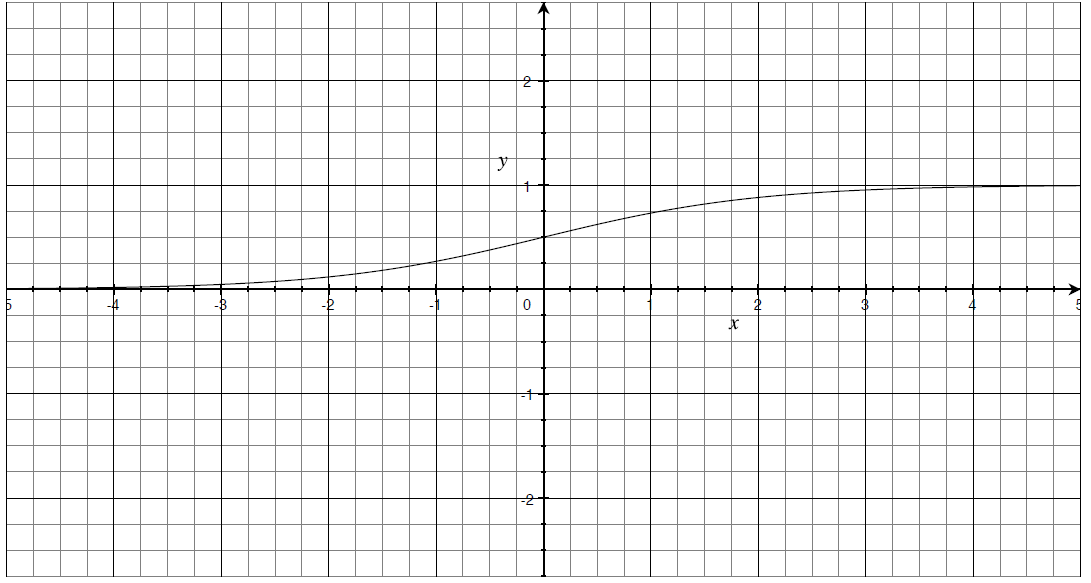
\includegraphics[width=0.6\linewidth]{Gambar/mine/sigmoid}
	\caption[Kurva Sigmoid, dari \cite{IntroNNforJava:2015}]{Kurva Sigmoid, dari \cite{IntroNNforJava:2015}} 
	\label{fig:k_sigmoid}
	\end{figure}
Hal penting yang perlu diperhatikan dalam menggunakan fungsi sigmoid. Fungsi ini hanya akan menghasilkan nilai positif.\\\\
\textbf{Hyperbolic Tangent}
Jika pada fungsi sigmoid y akan selalu selalu bernilai positif. Dengan menggunakan fungsi Hyperbolic Tangent maka nilai y bisa bernilai negatif. Jika keluaran yang kita ingin dapat bernilai negatif dan positif, kita dapat menggunakan fungsi Hyperbolic Tangent yang di definisikan sebagai berikut:
\begin{displaymath}
	f(x)=\frac{e^{2x}-1}{e^{2x}+1}
\end{displaymath}
Kurva \ref{fig:k_tangent} menggambarkan fungsi Hyperbolic Tangent dimana nilai y dapat bernilai positif atau negatif bergantung pada x yang diberikan.
\begin{figure}
	\centering
	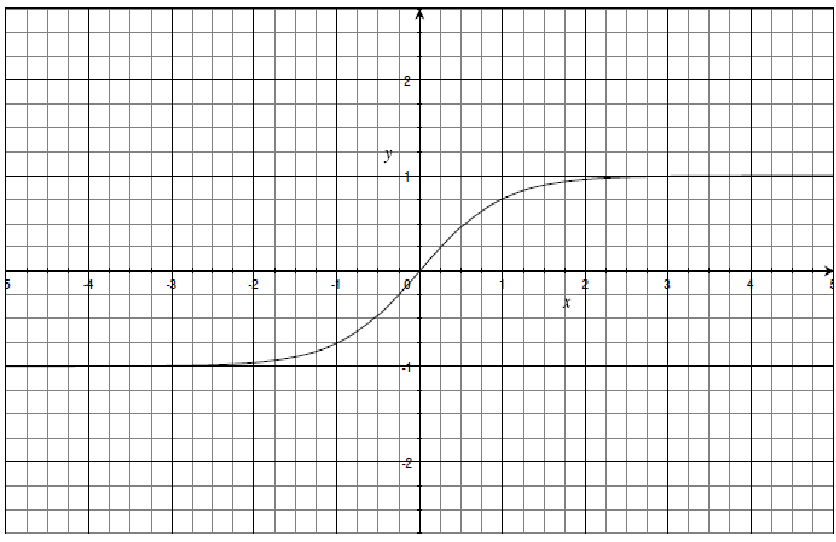
\includegraphics[width=0.6\linewidth]{Gambar/mine/tangent}
	\caption[Kurva Tangent, dari \cite{IntroNNforJava:2015}]{Kurva Tangent, dari \cite{IntroNNforJava:2015}} 
	\label{fig:k_tangent}
	\end{figure}
\end{enumerate}
\subsection{Backpropagation}
\textit{Backpropagation} adalah salah satu metode untuk melakukan pelatihan pada jaringan feedforward yang memiliki beberapa layer. \textit{Backpropagation} dapat digunakan untuk setiap jaringan feedforward yang menggunakan sebuah fungsi aktivasi yang dapat diturunkan. Pada backpropagation bobot setiap penghubung antar neuron akan dirubah agar JST dapat menghasilkan keluaran yang diharapkan sesedikit mungkin mengalami kesalahan.\\\\ 
\section{Database Management System}
\subsection{Fungsi dan karakteristik DBMS}
Secara tradisional pengorganisasian data biasanya dalam format file. Karena banyak kekurangan yang dimiliki dari pengorgansiasian tradisional (format file), maka dirancanglah sebuah konsep baru bernama Database Managment System (DBMS) untuk menutupi kekurangan penyimpanan tradisional \cite{DBMS:2015}.  Pada DBMS modern memiliki karakteristik sebagai berikut :
\begin{enumerate}
	\item \textbf{Real-world entity} : DBMS modern dirancang agar lebih realistik dengan menggunakan entitas yang berada di dunia nyata untuk merancang arsitekturnya. DBMS juga memiliki atribut dan kebiasaan dari entitas itu sendiri.
	\item \textbf{Relation-based tables} : DBMS memperbolehkan hubungan antar entitas kedalam bentuk tabel. Dengan hal tersebut pengguna dapat mengerti arsitektur dari basis data hanya dengan  melihat nama-nama tabelnya.
	\item \textbf{Isolation of data and application} : Sistem basis data seluruhnya berbeda dari datanya. Sebuah basis data adalah sebuah entitas aktif, sedangkan datanya adalah entitas pasif. DBMS menyediakan metadata, yaitu data mengenai data.
	\item \textbf{Less redundancy} : DBMS mengikuti peraturan normalisasi, dimana membagi sebuah relasi ketika atribut unik dari entitas tersebut memiliki nilai yang sama.
	\item \textbf{Consistency} : Konsistensi adalah status dimana setiap relasi dalam basis data tetap sesuai dengan yang seharusnya (tidak terjadi perubahan yang membingungkan). Pada DBMS ada beberapa metode dan teknik, yang dapat mendeteksi ketidak konsistenan data. 
	\item \textbf{Query Language} : DBMS diperlengkapi dengan bahasa query, yang membuat DBMS lebih efisien ketika ingin mendapatkan dan memanipulasi data.  
	\item \textbf{ACID Properties} : DBMS menerapkan perinsip \textbf{A}tomicity, \textbf{C}onsitency, \textbf{I}solation, \textbf{D}urabillity (Disingkat ACID). Dengan menerapkan prinsip ACID, membantu basis data tetap sehat dalam menangani banyak transaksi data. 
	\item \textbf{Concurrent Access} : DBMS mendukung multi-user dalam mengakses dan memanipulasi data dalam waktu yang bersamaan.
	\item \textbf{Security} : DBMS menawarkan banyak perbedaan level keamanan. Hal ini dapat membatasi setiap user dalam mengakses dan memanipulasi data.
\end{enumerate} 
\subsection{Data Model}
Data model mendefinisikan bagaimana struktur logika dari basis data di modelkan. Data model juga mendefinisikan bagaimana setiap data terhubung dengan yang lain dan bagaimana data diproses dan disimpan didalam sistem \cite{DBMS:2015}. Data model yang pertama kali digunakan adalah flat data-model, dimana semua data yang digunakan disimpan didalam tempat yang sama dan menyebabkan banyak duplikasi dan pembaruan yang anomali. Karena banyak kelemahan yang dimiliki flat data-model makan dirancang data model yang diharapkan lebih baik diantaranya :\\\\
\textbf{Entity-Relationship Model}\\
Entity-Relationship (ER) Model diciptakan berdasarkan karakteristik DBMS dari Real-World Entities dan hubungan antar entitasnya. Untuk memodelkan Real-World Entites kedalam DBMS dibutukah sebuah model konseptual, maka digunakanlah ER Model. Pada gambar \ref{fig:erd} menunjukan konsep ER Model.
	\begin{figure}
	\centering
	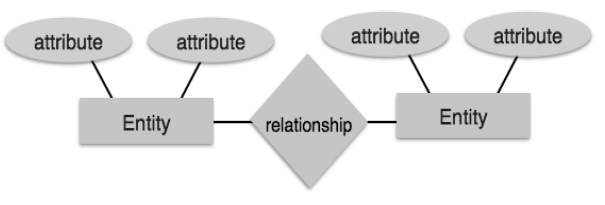
\includegraphics[width=0.6\linewidth]{Gambar/mine/erd}
	\caption[ER Model, dari \cite{DBMS:2015}]{ER Model, dari \cite{DBMS:2015}} 
	\label{fig:erd}
	\end{figure}
\begin{enumerate}
	\item \textbf{Entity}\\
	\textit{Entity} atau entitas dalam ER Model adalah sebuah entitas di dunia nyata yang memiliki sifat disebut \textbf{attribute} atau atribut. Setiap atribut di definisikan oleh sekumpulan nilai yang disebut \textbf{domain}.
	\item \textbf{Relationship}\\
	Asosiasi logika antar entitas disebut \textbf{relationship}. Relationship dipetakan dengan entitas dengan cara yang bervariasi. Untuk memetakan kardinalitas antar entitas dapat didefinisikan dengan angka dari asosiasi diantara kedua entitas. Jenis pemetaan kardinalitas diantaranya \textit{one to one, one to many, many to one, many to many}.
\end{enumerate}
\textbf{Relational Model}\\
Relational model adalah pengorganisasian data kedalam sekumpulan tabel yang datanya dapat di akses atau dirakit kembali kedalam banyak cara tanpa harus melakukan organisasikan kembali pada tabel database Gambar \ref{fig:relational} menunjukan contoh relational model \cite{RelationDefinition:2001}. Setiap table (atau kadang disebut relasi) mengandung satu atau lebih kategori data dalam kolom (\textit{attribute}). Setiap baris (\textit{tuples}) mengandung instansiasi yang unik dari data. Keuntungan menggunakan relational model daripada model lainya :
\begin{enumerate}
	\item Berdasarkan pengertian matematika relasi dan himpunan, sehingga dapat menggunakan abstraksi matematika.
	\item Menggunakan struktur data yang sederhana, mudah dimengerti.
	\item Membagi level logis dan level fisikal. 
	\item Operasi tidak perlu mengerti struktur data yang digunakan.
\end{enumerate}
	\begin{figure}
	\centering
	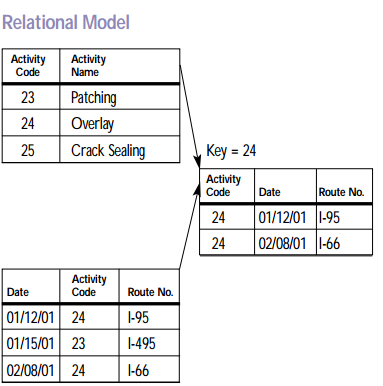
\includegraphics[width=0.6\linewidth]{Gambar/mine/relational}
	\caption[Model Relational, dari \cite{RelationDefinition:2001}]{Model Relational, dari \cite{RelationDefinition:2001}} 
	\label{fig:relational}
	\end{figure}
\subsection{SQL}
SQL kepanjangan dari Structured Query Language adalah sebuah bahasa standard untuk mengakses dan memanipulasi basis data. SQL adalah sebuah standard ANSI(American National Standards Institute). Dengan menggunakan \textit{statement} SQL kita dapat memanipulasi sebuah basis data. Setiap \textit{statement} memiliki sintaksis. Berikut beberapa sintaksis dasar dan fungsinya :
\begin{enumerate}
	\item SELECT columnNname, columnNname FROM tableName WHERE columnName operator value \\ Berfungsi mengambil data berdasarkan kolom dari sebuah Tabel dengan kondisi dimana nilai dari column tersebut memenuhi suatu nilai.
	\item INSERT INTO tableName VALUES value1,value2,value3,...\\
Berfungsi memasukan nilai-nilai kedalam sebuah table atau relasi.
	\item UPDATE tableName SET column1=value1,column2=value2,... WHERE someColumn=someValue\\
Berfungsi merubah nilai-nilai pada sebuah table di sebuah \textit{tuple} yang memenuhi sebuah kriteria
	\item DELETE FROM tableName WHERE someColumn=someValue\\
	Berfungsi menghapus sebuah \textit{tuple} yang memiliki kriteria tertentu
\end{enumerate}
\subsection{MySQL}
MySQL adalah salah satu Relational DBMS \textit{open source} yang paling populer di dunia. MySQL dapat membantu pengembang mendapatkan aplikasi basis data yang memiliki performa tinggi, \textit{scalable} dan \textit{cost-effectively}. MySQL menyediakan edisi gratis dan komersial. Edisi Gratis MySQL dapat diunduh bersama Apache dan PHP dalam paket XAMPP di situs \url{https://www.apachefriends.org/index.html}.
\subsection{JDBC}
JDBC adalah sebuah API yang di rancang untuk menghubungkan basis data SQL dengan pemograman berbahasa Java. JDBC menyediakan metode untuk melakukan \textit{query} dan \textit{updating} data kedalam database. JDBC berorientasi dengan basis data relasional. Berikut beberapa kelas yang dimiliki oleh JDBC:\\
\textbf{Connection} adalah sebuah interface yang berfungsi melakukan koneksi dengan sebuah spesifik basis data. Method yang dimiliki kelas ini sebagai berikut:
\begin{enumerate}
	\item \textbf{Statement createStatement()}\\
	Berfungsi membuat sebuah objek Statement untuk mengirimkan SQL statments kedalam basis data.\\
	\textbf{Kembalian} Statement
	\item prepareStatement(String sql)
	Berfungsi membuat objek PrepareStatement untuk mengirimkan parameter SQL kedalam database.\\
	\textbf{Parameter} sql - String
	\textbf{Kembalian} sebuah objek PreparedStatement
\end{enumerate}
\textbf{DriverManager} Layanan dasar untuk mengelola satu set JDBC driver. Method yang dimiliki kelas ini sebagai berikut:
\begin{enumerate}
	\item \textbf{Connection getConnection(String url)}\\
	Berfungsi mendapatkan objek Connection
	\textbf{Parameter} url - String\\
	\textbf{Kembalian} objek Connection
\end{enumerate}
\textbf{PreparedStatement} Adalah sebuah kelas yang merepresentasikan sebuah \textit{precomplied SQL statment}. Method yang dimiliki kelas ini sebagai berikut:
\begin{enumerate}
\item \textbf{void Execute()}
Berfungsi melakukan eksekusi terhadap query
\textbf{Kembalian} void
\end{enumerate}
\textbf{Statement} Adalah sebuah interface yang berfungsi mengeksekusi perintah SQL statik dan mengembalikan hasil perintah tersebut. Method yang dimiliki kelas ini sebagai berikut:
\begin{enumerate}
	\item \textbf{ResultSet executeQuery(String sql)}\\
	Berfungsi mengeksekusi perintah SQL yang diberikan.\\
	\textbf{Parameter} sql - String
	\textbf{Kembalian} sebuah objek ResultSet
\end{enumerate}